%%%%%%%%%%%%%%%%%%%%%%%%%%%%%%%%%%%%%%%%%%%%%%%%%%%%%%%%%%%%%%%%%%%%%%%%%%%%%%%%
%2345678901234567890123456789012345678901234567890123456789012345678901234567890
%        1         2         3         4         5         6         7         8

\documentclass[letterpaper, 10 pt, conference]{ieeeconf}  % Comment this line out
\usepackage{hyperref}
                                                          % if you need a4paper
%\documentclass[a4paper, 10pt, conference]{ieeeconf}      % Use this line for a4
                                                          % paper

\IEEEoverridecommandlockouts                              % This command is only
                                                          % needed if you want to
                                                          % use the \thanks command
\overrideIEEEmargins
% See the \addtolength command later in the file to balance the column lengths
% on the last page of the document



% The following packages can be found on http:\\www.ctan.org
\usepackage{graphicx} % for pdf, bitmapped graphics files
\usepackage[figurename=Figure ]{caption}
%\usepackage{epsfig} % for postscript graphics files
%\usepackage{mathptmx} % assumes new font selection scheme installed
%\usepackage{times} % assumes new font selection scheme installed
%\usepackage{amsmath} % assumes amsmath package installed
%\usepackage{amssymb}  % assumes amsmath package installed
\usepackage{subfig}
\title{\LARGE \bf
The Effect of Genetic Connectivity on the Strength of Natural Selection in \textit{Chlamydomonas reinhardtii }
}

%\author{ \parbox{3 in}{\centering Huibert Kwakernaak*
%         \thanks{*Use the $\backslash$thanks command to put information here}\\
%         Faculty of Electrical Engineering, Mathematics and Computer Science\\
%         University of Twente\\
%         7500 AE Enschede, The Netherlands\\
%         {\tt\small h.kwakernaak@autsubmit.com}}
%         \hspace*{ 0.5 in}
%         \parbox{3 in}{ \centering Pradeep Misra**
%         \thanks{**The footnote marks may be inserted manually}\\
%        Department of Electrical Engineering \\
%         Wright State University\\
%         Dayton, OH 45435, USA\\
%         {\tt\small pmisra@cs.wright.edu}}
%}

\author{Sara El-Shawa$^{1}$ and Rob W Ness$^{1, 2}$% <-this % stops a space
\thanks{$^{1}$Department of Biology, University of Toronto Mississauga, Mississauga, Canada
        {\tt\small}}%
\thanks{$^{2}$Department of Ecology and Evolutionary Biology, University of Toronto, Toronto, Canada
        {\tt\small }}%
}


\begin{document}



\maketitle
\thispagestyle{empty}
\pagestyle{empty}


%%%%%%%%%%%%%%%%%%%%%%%%%%%%%%%%%%%%%%%%%%%%%%%%%%%%%%%%%%%%%%%%%%%%%%%%%%%%%%%%
\begin{abstract}

Genetic networks can represent the complex biological interactions amongst genes, proteins and metabolites. Numerous advances have demonstrated the power of genetic networks to model and predict the effects of gene knock-outs and other mutations. While such experimental studies are important, evolutionary genetics research is only beginning to utilize networks to understand the consequences of mutations on fitness and how networks have evolved. Within a genetic network, the interconnectivity of genes can vary. Genes that are highly connected to other genes have more interactions and therefore may be subject to more functional constraints. We predict that network connectivity of genes will affect the strength of selection on them. In this study, we examine the influence of natural selection on genes across a genetic network of \textit{Chlamydomonas reinhardtii}. This was done by calculating the level of synonymous and non-synonymous diversity and divergence for each gene in the network. We then correlated the network properties for each gene (e.g. connectivity) with diversity and divergence. We present results that demonstrate how the position of a gene in a network influences the strength and direction of natural selection. We found that connectivity has no effect on divergence and a negative correlation with diversity. 

Keywords: Genetic Networks, Natural Selection, Genetic Diversity, Genetic Divergence, Connectivity
\end{abstract}
% \hyperlink{MyTargetKey}{\cite{c1}}

%%%%%%%%%%%%%%%%%%%%%%%%%%%%%%%%%%%%%%%%%%%%%%%%%%%%%%%%%%%%%%%%%%%%%%%%%%%%%%%%
\section*{\normalfont{\textbf{\fontsize{13}{6}\selectfont Background}}}

\setlength{\parindent}{10ex} Evolutionary rates of proteins are known to be highly variable and can be better understood through the investigation of different selective constraints which are present in a given environment. In the case of positive selection, advantageous genetic variants persist, whereas when proteins are under negative selection, deleterious genetic variants are removed. It is a challenge to successfully predict the strength of selection through studying an individual protein in isolation. Analyzing proteins as a part of a biological pathway can reveal insights into evolutionary rates when we consider that most proteins are connected to other proteins within functional pathways. 

\setlength{\parindent}{10ex} Previous studies on specific biological pathways such as the anthocyanin biosynthetic pathway (ABP) genes have shown that genes at an earlier position in a pathway such as CHS are subject to higher selective pressures when compared to downstream genes such as UFGT wherein the selective pressures are weaker and evolutionary rates are increased \cite{rmt99}. From these studies, we can note how genes in different positions along a single biochemical pathway experience variability in their respective selective pressures. This notion may still apply when scaled up to entire biological networks; the complete representation of all interactions between pathways. Gene regulatory, protein interaction, and metabolic networks are all examples of networks that are used to represent different kinds of biological interactions. 

\setlength{\parindent}{10ex} 
Genetic networks are used at different levels to study biological interactions. One type of network, the metabolic network, consists of nodes which represent metabolites or proteins and are connected by edges which represent enzymatic reactions. Metabolic networks can become extremely complex in the presence of numerous feedback loops and cellular subnetworks within them. This degree of complexity renders experimental techniques alone inefficient for deeper level analysis, thus requiring an approach that integrates computational modelling. 


\setlength{\parindent}{10ex} Each individual component of a genetic network must be analyzed by looking at information including the activities and kinetic parameters of enzymes, the absolute concentration of metabolites, as well as fluxes \cite{Stitt428}. Moreover, in a genetic network, one metabolite typically requires the operation of several pathways, and groups of metabolites are normally synthesized simultaneously. Therefore, analyzing a network should not only be done by dividing the network into discrete pathways \cite{Stitt428}. A complete thorough analysis of a network must account for all interactions. Studying specific network modules in a genetic network will aid in understanding how genetic changes lead to other developmental changes or mutations \cite{Wilkins8590}. 

\setlength{\parindent}{10ex} Identifying influential nodes in a network is advantageous for a variety of applications. A study looking at the \textit{S. cerevisiae} protein-protein interaction network found that the deletion of a gene encoding a highly connected protein resulted in a large impact on the network. There was a positive correlation between lethality and connectivity, suggesting that highly connected nodes are essential for the survival of the organism \cite{jmbo01}. Furthermore, another study examining the \textit{E. coli} metabolic network found that the most connected nodes, glutamate and pyruvate, are some of the oldest nodes phylogenetically. This is explained by the growth of metabolic networks over the course of evolutionary time through the addition of new metabolites to pathways. Therefore, these older nodes are at the core of the most ancient metabolic pathways and consequently, are essential components of the network structure \cite{fw00}.

\setlength{\parindent}{10ex}The degree of a node, or the number of links one node has to other nodes, is a basic local centrality measure \cite{bo04}. Connectivity is defined as the degree of connections a node has in a genetic network. One way to analyze a genetic network is to find the relationship between connectivity and gene essentiality. Highly connected nodes are predicted to have a higher relative importance in the network. \cite{carl} analyzed the \textit{Saccharomyces} genome, \textit{Neurospora} genome, \textit{Drosophila} genome, and \textit{C. elegans} genome and found that there is a positive correlation between gene connectivity and gene sequence conservation as well as gene essentiality across the entire genetic network between species. Moreover, a study looking at the protein-protein interaction networks in \textit{Saccharomyces cerevisiae, Caenorhabditis elegans}, and \textit{Drosophila melanogaste} found that degree centrality is significantly higher in essential proteins across all three networks \cite{hk04}. This suggests that highly connected nodes posses greater essentiality in the network. 

\setlength{\parindent}{10ex}
The genome-scale metabolic network of \textit{C. reinhardtii} (iRC1080) that was reconstructed in 2011 is ideal for the analysis of selection in genetic networks \cite{Chang1}. Since \textit{C. reinhardtii} is a unicellular green alga, its genome is far less complicated than other multicellular eukaryotes \cite{Merchant245}. The iRC1080 network consists of 2190 reactions and 1068 metabolites that are associated with 1080 genes \cite{Chang1}. \textit{Chlamydomonas} is a model genus of eukaryotic microalgae that is used to study various biological processes, and \textit{C. reinhardtii} is the predominant laboratory species of this genus and green algae in general \cite{eliz}. 

\setlength{\parindent}{10ex}
The present study aims to analyze the interactions of the genetic network, rather than just the sequences. One core analysis this present study targets is quantifying the connectivity and selection in the iRC1080 genetic network and analyzing the relationship between those two variables. It is predicted that genes that have a large role in the network will be less vulnerable to selection than those that have a smaller role. Genes with high connectivity are predicted to have an increased effect of purifying selection compared to genes with low connectivity.  This is due to highly connected nodes in the network which are more likely to be essential for the survival of the organism. It is greatly probable for selection to act against a mutation in a highly connected gene since there would be a larger consequence on the network and genome.



\section*{\normalfont{\textbf{\fontsize{13}{6}\selectfont Methods}}}

\setlength{\parindent}{10ex} To conduct analyses of selection, we need to first estimate the diversity and divergence properties of each gene in the network. Sequence divergence accounts for inter-specific differences and is the accumulation of independent genetic changes through time between two organisms. Diversity, on the other hand, accounts for intra-specific differences. \textit{C.incerta}, \textit{C. reinhardtii} most closely related sister species was used to estimate divergence. Sequences that are under high selective constraints (purifying selection) will have relatively few changes in \textit{C. reinhardtii} and \textit{C. incerta}, and, therefore, will have low divergence. Furthermore, sequences within \textit{C. reinhardtii} that are under high selective constraints will have low diversity.  Sequences that are under positive selection will be highly divergent between \textit{C. incerta} and \textit{C. reinhardtii}. We then studied the relationship between connectivity with divergence and diversity, separately. 


\subsection*{\normalfont{\textbf{Annotating \textit{C. Incerta} and \textit{C. reinhardtii} genes}}}
For the present study, we used the \textit{C. incerta} draft genome to estimate divergence which was received from Rob Ness (personal communication) since it is the most closely related species to \textit{C. reinhardtii}. We then used Augustus gene annotator on the \textit{C. incerta} draft genome to predict its genes \cite{sm05}. Furthermore, version 5.3 of the \textit{C. reinhardtii} reference genome was used in the current study. The reference genome is available for download on phytozome.net \cite{gshnhf}.

\subsection*{\normalfont{\textbf{Identifying Orthologs}}}
To identify homologous genes between \textit{C. incerta} and \textit{C. reinhardtii}, the Reciprocal Best Hits (RBH) were identified. This ensues when two genes, one in the \textit{C. incerta} draft genome and the other in the \textit{C. reinhardtii} reference genome, have one another as their best scoring match. Although NCBI’s BLAST is most commonly used to find RBH, it was found that UBLAST was a better option due to its speed and accuracy \cite{wm14}. Therefore, we first applied USEARCH to create databases out of each organism’s reference protein sequences in fasta format \cite{e10}. Then, we used UBLAST to identify homologs in the reciprocal best hit framework \cite{e10}.     

\subsection*{\normalfont{\textbf{Bacteria in \textit{C. Incerta} Genome}}}
The \textit{C. incerta} genome used in this study was a draft genome, bringing about the possibility that contamination of algal cultures could be present within the DNA that was sequenced. To identify genes from the RBH that were bacteria, we BLASTed hits with percent identity (pid) less than 90\% and query coverage (qcovs) less than 90\% against the non-redundant (NR) protein database.  
 


\subsection*{\normalfont{\textbf{Aligning Exons}}}
Since exons encode for proteins, they are under higher selective pressure than other components of the gene. Therefore, we did not align the entire gene at once as the intron alignments would complicate the exon alignments. The first step in the process was the exon alignment. This was done by translating the sequences into protein, aligning the translated sequences using MUSCLE \cite{e04}, and reversing the alignments back to DNA alignments (see supplementary data for code).  Although Anchored DIALIGN is a tool that forces certain regions (in our case, the exons) to correctly align and then aligns the remainder of the sequences under those constraints, the program requires the anchors to be of equal length of both sequences \cite{mpps06}. Since several RBH had different number of coding sequences between homologs due to an intron insertion mutation in one of the coding sequences, we continued the study with exon alignments only. 


\subsection*{\normalfont{\textbf{Estimating Evolutionary Distance}}}
The change of DNA sequences through evolution occurs through three processes: insertions, deletions, and nucleotide substitutions. To measure the rate of divergence in \textit{C. reinhardtii}, we estimated the number of synonymous ($d_S$)  and non-synonymous ($d_N$) substitutions per site between two sequences \cite{yn00}. This was done by using the alignments of homologous pairs of \textit{C. incerta} and \textit{C.reinhardtii} genes. Three steps were taken to estimate the evolutionary distance between the two \textit{Chlamydomonas} species. First, the total number of synonymous and non-synonymous sites in the homologs were counted. Second, the number of differences of synonymous and non-synonymous sites between the homologs were counted. Lastly, a method of correction for multiple substitution at the same site was applied \cite{yn00}. We used the simple Jukes and Cantor’s method to convert the observed difference to an estimate of evolutionary divergence, using the following equation: 

$$
d = -\frac{3}{4}\log_e(1-\frac{4}{3}p)  \eqno{(1)}
$$


where $p$ is the proportion of sites with different nucleotides \cite{jc69}. We then quantified the strength of selective pressure by calculating $w$, the ratio of non-synonymous to synonymous DNA substitutions. The reason behind this is to take into account the variation in the underlying mutation rate when reporting the variation in non-synonymous divergence \cite{h02}.

$$
w = \frac{d_N}{d_S}  \eqno{(2)}
$$


\subsection*{\normalfont{\textbf{Estimating Diversity}}}
Diversity was estimated by calculating the site frequency spectrum (SFS) at synonymous (4-fold degenerate) and non-synonymous (0-fold degenerate) sites. This was done by counting the frequency of the minor allele at each site. Theta pi ($\theta \pi$) was then calculated as the average number of pairwise nucleotide differences per site to quantify diversity at synonymous and non-synonymous sites.

\section*{\normalfont{\textbf{\fontsize{13}{6}\selectfont Results}}}

The output of the gene finder AUGUSTUS contained 31,675 \textit{C. incerta} genes in gff format along with the coding sequences and protein sequences of each gene. However, more than half of the \textit{C. incerta} genes found by AUGUSTUS were disposed of, since only 12,926 RBHs were identified. We studied two variables, pid and qcovs, to analyze the distribution of the RBH output. Furthermore, the BLAST output against all known proteins found that from these 12,926 genes, 17 of them had bacteria genes as their best scoring match.

\setlength{\parindent}{10ex} 
All 12,926 RBH had their exons aligned. One fasta file contains all exon alignments, where each two alignments represent a pair of RBH consisting of a \textit{C. incerta} gene and a \textit{C. reinhardtii} gene (see supplementary data). Before proceeding with calculating divergence and diversity rates, only genes that were present in the iRC1080 network were taken. Then, alignments of these genes were manually viewed and discarded if they were low quality alignments. Alignments were considered low quality if they did not have a long stretch of matching nucleotides and appeared to be random. A final total of 583 genes that were in the iRC1080 network were used for the analysis of divergence and diversity.



\subsection*{\normalfont{\textbf{Quantifying Connectivity}}}
In the iRC1080 network, each node has a descriptive name that is associated with a “gene reaction rule” \cite{kldmfl}. This contains the name of a gene that a specific node interacts with. Some genes were found to be a part of multiple gene reaction rules, and therefore, had more than one node in the network represent them. This led to one gene having multiple measures of connectivity. Since we are studying the effect of connectivity, we used the maximum degree of each gene that is related to multiple nodes for our study. The degree measurement varied from only two connected neighbors (low connectivity) up until nine connected neighbors (high connectivity) (Table 1).

\subsection*{\normalfont{\textbf{Measuring Diversity and Divergence}}}
The average $\theta \pi_S$ value for SFS at 4-fold degenerate sites was 0.023 with values ranging from 0.0 to 0.067 and a variance equaling to 0.000155. The average $\theta \pi_N$ value for SFS at 0-fold degenerate sites was 0.0022 with values ranging from 0.0 to 0.039 and a variance equaling to 8.8 e-06 (Table 1). On average, $\theta \pi_S$ was greater than $\theta \pi_N$, and the mean ratio of  $\theta \pi_N/\theta \pi_S$ was 0.09 ranging from values of 0.0 to 1.478. 

\setlength{\parindent}{10ex}
The average $d_N$ at 0-fold degenerate sites was 0.064 with values ranging from 0.0 to 2.34 and a variance equaling to 0.0380. The average $d_S$ at 4-fold degenerate sites was 0.253 with values ranging from 0.0271 to 0.41 and a variance equaling to 0.0071 (Table 1). Synonymous sites had greater divergence compared to non-synonymous sites, and the mean ratio of $d_N/d_S$ was 0.156 ranging from values of 0.0 to 0.595. All genes studied had a $d_N/d_S$ value of less than 1. 

   \begin{figure}[thpb]
      \centering
%       \framebox{{
%             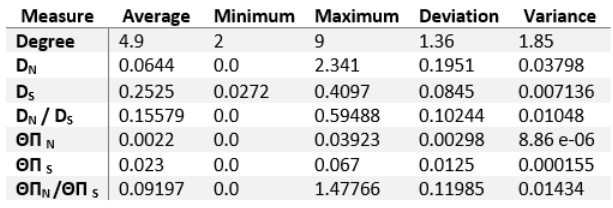
\includegraphics[scale=0.70]{table_thesis.PNG}

%             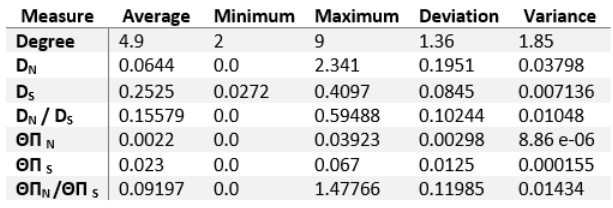
\includegraphics[scale=1.0]{table_thesis.PNG}

% }}
      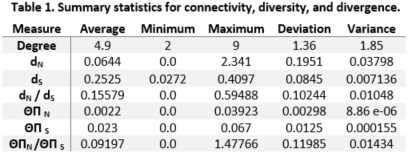
\includegraphics[scale=0.9]{newest_thesis_table.PNG}
   {\fontsize{7.5}{11}\selectfont Results of measuring connectivity and quantifying selection in iRC1080 genes}
      \label{hello i am testing}
   \end{figure}


 \begin{figure}[thpb]
      \centering
%       \framebox{{
%             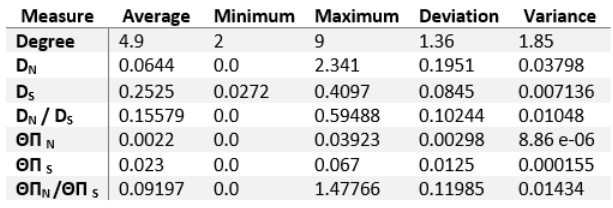
\includegraphics[scale=0.70]{table_thesis.PNG}

%             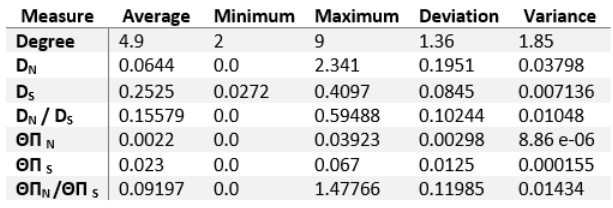
\includegraphics[scale=1.0]{table_thesis.PNG}

% }
      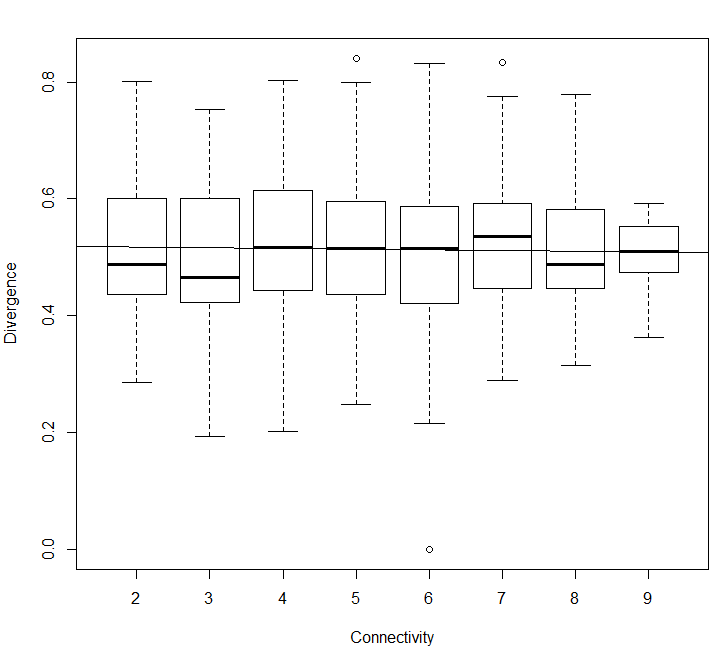
\includegraphics[scale=0.44]{final__divergence_connectivity.png}
      \caption{\fontsize{8}{11}\selectfont No variation in divergence between connectivity levels. Divergence ($w$ = $d_N/d_S$) for each gene in the iRC1080 network, categorized based on maximum degree of gene. The boxes outline the first to third quartile of divergence estimate from a given degree of connectivity, the horizontal lines within the boxes indicate the median divergence rate, and points within 1.5x the interquartile range are covered by whiskers. All other points lie beyond the whiskers. }
   \end{figure}
   

   

\subsection*{\normalfont{\textbf{Effect of Connectivity on Divergence and Diversity}}}

\setlength{\parindent}{10ex} We find that there is a negative correlation between $d_S$ and connectivity as well as $d_N$ and connectivity (one-way ANOVA p$<$0.001 and one-way ANOVA p$<$0.05, respectively). However, there is no effect of connectivity on divergence as a whole when $d_N/d_S$ is used as a measurement of divergence (one-way ANOVA p=0.778) (Figure 1).
 \begin{figure}[thpb]
      \centering
%       \framebox{{
%             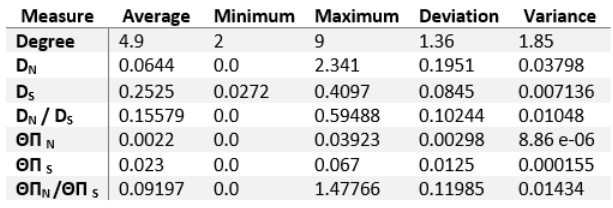
\includegraphics[scale=0.70]{table_thesis.PNG}

%             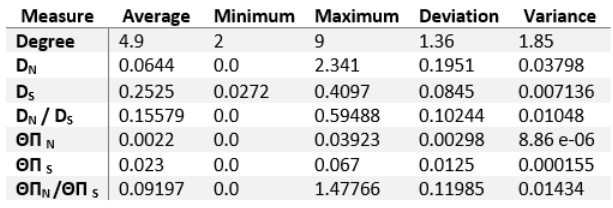
\includegraphics[scale=1.0]{table_thesis.PNG}

% }
      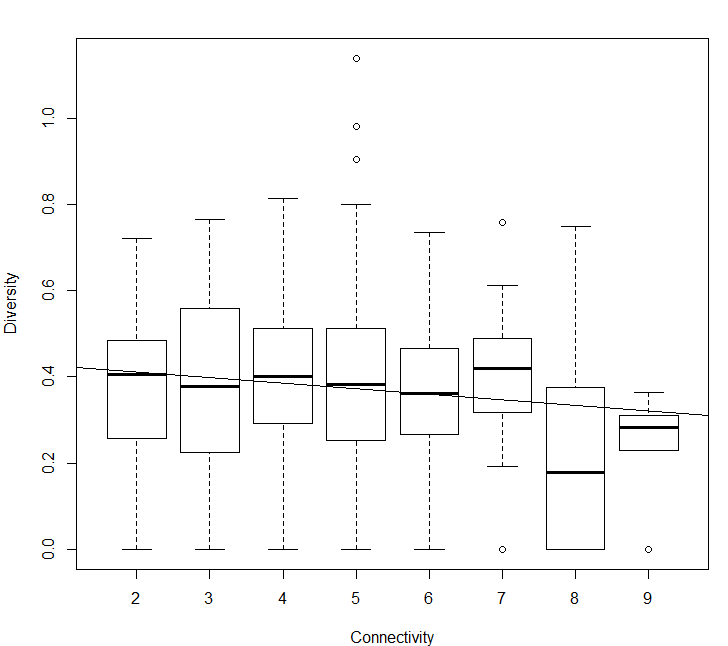
\includegraphics[scale=0.44]{FINAL_DIVERSITY_PLOT.png}
      \caption
      {\fontsize{8}{11}\selectfont Variation in diversity between connectivity levels. Diversity ($\theta \pi_N/\theta \pi_S$) for each gene in the iRC1080 network, categorized based on maximum degree of gene. The boxes outline the first to third quartile of diversity estimate from a given degree of connectivity, the horizontal lines within the boxes indicate the median diversity rate, and points within 1.5x the interquartile range are covered by whiskers. All other points lie beyond the whiskers. }
   \end{figure}   

\setlength{\parindent}{10ex} We find that there is a negative correlation between $\theta \pi_S$ and connectivity as well as $\theta \pi_N$ and connectivity (one-way ANOVA p=0.0137 and one-way ANOVA p$<$0.0185, respectively). Furthermore, there is a statistically significant result between the correlation of connectivity on diversity as a whole when $\theta \pi_N/\theta \pi_S$ ratio is used as a measurement of diversity (one-way ANOVA p$<$0.05) (Figure 2).


\section*{\normalfont{\textbf{\fontsize{13}{6}\selectfont Discussion}}}


583 genes in the iRC1080 shared orthologous sequences with \textit{C. incerta} as well as a measure of divergence and diversity at both synonymous and non-synonymous sites. The average degree of connectivity of a node was 4.9, and the maximum connectivity for each node variable ranged from two nodes to nine nodes with a standard deviation of 1.36. The effect of connectivity on the level of divergence at synonymous and non-synonymous sites was determined to be non-significant. However, we did find a significant negative correlation between connectivity and the level of diversity at synonymous and non-synonymous sites. I will be further discussing the implications of these two findings in greater detail.


\subsection*{\normalfont{\textbf{Alignment of Orthologs}}}
Out of the 1,080 genes present in the \textit{C. reinhardtii} network, approximately 54\% were retained for use in this study. The absence of approximately half of the initial genes can be attributed to multiple reasons. Firstly, the genes may not have had an orthologous sequence to \textit{C. incerta}, and therefore, rate of divergence could not be measured. The reciprocal best blast used to identify the orthologs could have discarded multiple \textit{C. reinhardtii} genes that did not have a good quality hit. Furthermore, orthologs that were identified by blast and aligned could be incorrect since the blast might not have been sensitive enough. Some of the alignments (approximately 200) were discarded due to inaccurate alignment measures. The reason why some RBH pairs which had a high pid and qcovs ultimately resulted in bad alignments could be due to blasting error. It is possible that the blast hit was very high on a small portion of the sequence such as a motif, and therefore, resulted in a high pid. Although a blast hit had a high pid, the rest of the sequence outside of the motif did not align properly, and therefore, resulted discarding these sequences. 


\subsection*{\normalfont{\textbf{Divergence}}}
Our estimate of divergence rate at synonymous sites is 0.68-fold lower than the estimate of a previous study in \textit{C.reinhardtii} \cite{pl07}. This decrease in average divergence could be due to the earlier disregard of some alignments. Furthermore, the estimate of divergence rate at non-synonymous sites is 3.58-fold higher than the estimate of the same previous study \cite{pl07}. As for the $d_N/d_S$, our estimate of 0.15579 is 2.78-fold higher. Although our specific measures did not accurately match other studies, the general trend of having a higher divergence rate at synonymous sites compared to non-synonymous sites is clearly shown. Synonymous sites are under weaker selective constraint, and therefore are able to diverge at a higher rate. 

The rate of strength of selection can be divided into 3 groups of measurement of $d_N/d_S$ or $w$. Firstly, if $w$=1, this means that an amino acid change (non-synonymous) is neutral and will have the same fixation rate as a synonymous change. $w$ $<$ 1 if non-synonymous changes are deleterious due to purifying selection. Lastly, if $w$ $>$ 1, this means that non-synonymous changes are advantageous and are under positive selection \cite{yb00}. Since all genes had a measurement of $w$ $<$ 1, this means that the all genes studied in the iRC1080 are being acted upon by purifying selection, however, the strength of purifying selection differs between genes. 


 

\setlength{\parindent}{10ex}
We expected to see a negative correlation between connectivity and divergence at non-synonymous sites, since highly connected nodes were predicted to be under stronger selective constraint. We also expected to see no correlation between connectivity and divergence at synonymous sites, seeing as synonymous site divergence cannot change the amino acid.Through a one-way ANOVA, we found that for both synonymous and non-synonymous sites, there was a significant effect of connectivity on divergence. We did not find a significant effect of connectivity on $d_N/d_S$ ratio. A reduction in both synonymous and non-synonymous divergence as connectivity increases might be perhaps due to a lower mutation rate on synonymous sites. Synonymous divergence rate has been extensively studied in \textit{E. coli} and \textit{S. typhimurium}. Berg (1999) found that the variation in synonymous divergence is due to spontaneous mutation rates at specific sites \cite{b99}. Furthermore, Sharp (1991) examined the determinants of sequence divergence between the same two organisms and found that factors such as codon usage and chromosomal location significantly varied rate of synonymous divergence \cite{s91}.  

\begin{figure}[!tbp]
  \centering
  \subfloat[Diversity at synonymous sites]{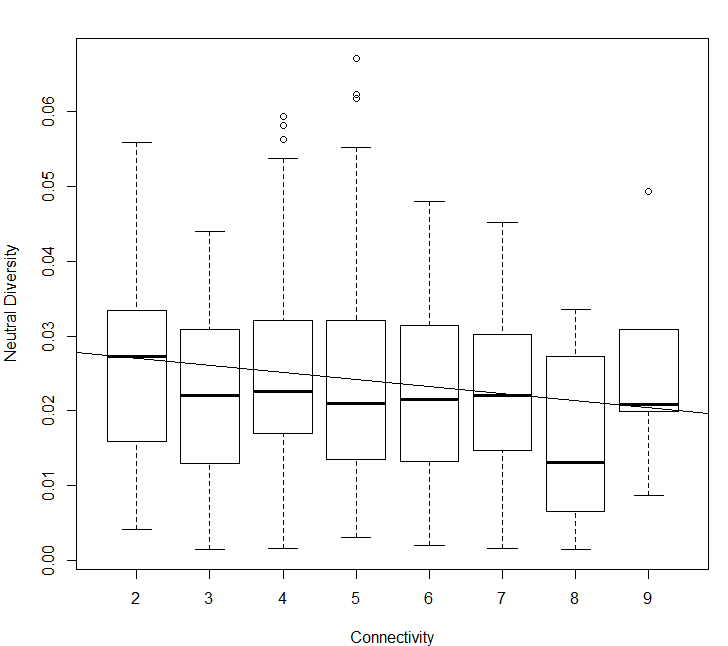
\includegraphics[width=0.44\textwidth]{neutral_diversity_final.png}\label{fig:neutral diversity}}
  \hfill
  \subfloat[Diversity at non-synonymous sites.]{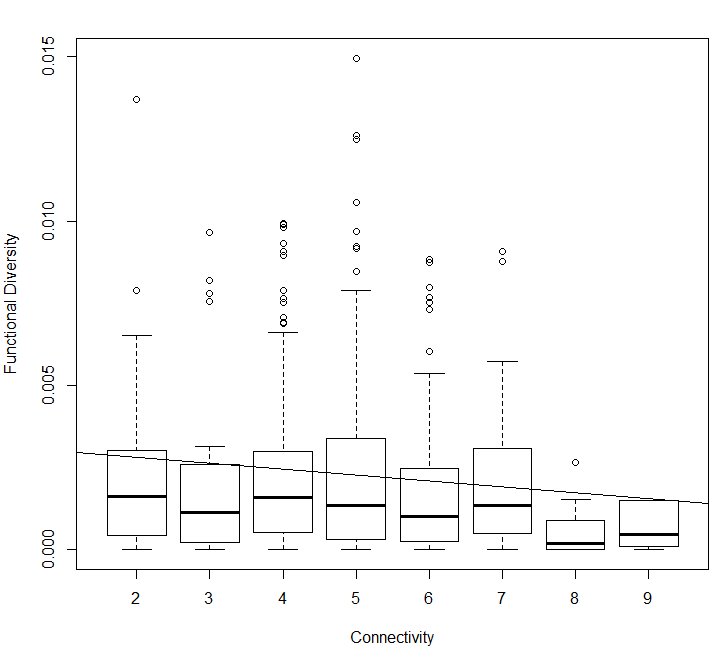
\includegraphics[width=0.44\textwidth]{functional_diversity_final.png}\label{functional diversity}}
  \caption{\fontsize{8}{11}\selectfont Variation in different sites of diversity between connectivity levels. Difference in slopes between diversity at neutral sites ($\theta \pi_S$) and diversity at functional sites ($\theta \pi_N$) for each gene in the iRC1080 network, categorized based on maximum degree of gene.}
\end{figure}

\subsection*{\normalfont{\textbf{Diversity}}}
The average measure of diversity $\theta \pi_S$ is 0.023, whereas the $\theta \pi_N$ has an average of 0.0022. This supports our prediction that synonymous sites are under weaker selective constraints and therefore exhibit higher diversity. The average rate of diversity of $\theta \pi_N/\theta \pi_S$ is 0.091967. It is hypothesized that diversity will decrease with increasing selection even in synonymous sites due to linked selection \cite{eshsma}. Diversity at both synonymous and non-synonymous sites were negatively correlated with connectivity. Furthermore, as expected, we find a negative correlation between $\theta \pi_N/\theta \pi_S$ and connectivity, with highly connected nodes having a lower diversity rate in comparison to nodes with few connections. We expect that although both synonymous and non-synonymous sites exhibit a negative correlation with connectivity, non-synonymous sites should show a stronger correlation. To test this, we performed an ANOVA to test the difference of slopes between the different sites (Figure 1). The result was statistically significant (p $<$ 0.05), showing that the change in rate of diversity is not the same in synonymous and non-synonymous sites.  

Although a slight pattern is seen in studying diversity and connectivity, there is no effect on overall divergence. One explanation for this phenomenon is supported by a study where divergence and diversity selection was examined in \textit{P. mexicana} and found that selection favours diversity within species but not divergence between species \cite{tprsgm}. For example, a gene's diversity can change as it gets added to/removed from the population, and this occurs higher or lower in frequency depending on the connectivity of the node. However, due to selection, the gene never ultimately gets to a point of divergence. Therefore, we see a change in diversity but not in divergence. 
\setlength{\parindent}{10ex}

% Although a slight pattern is seen in studying diversity and connectivity, there is no effect on overall divergence. This can be explained by a multitude of reasons. One idea is that a gene can be more or less diverse, as it get removed from the population, and this occurs higher or lower in frequency depending on the connectivity of the node. However, the gene never ultimately gets to a point of divergence since selection is strong in all genes. Therefore, we see a change in diversity but not in divergence.


\subsection*{\normalfont{\textbf{Future Directions}}}


To understand the distribution of fitness effects (DFE), we can apply DFE-alpha to polymorphism and divergence data of genes in the iRC1080 network. DFE-alpha can be used to estimate the fraction of sites that are under negative selection \cite{ek09, ke07, kk13}. This program will be a more accurate measure of selection than the conventional method of calculating $\theta \pi_N/\theta \pi_S$ and  $d_N/d_S$. Using DFE-alpha, we can test whether or not highly connected genes evolve more adaptive changes per mutation compared to low connected genes. 

\setlength{\parindent}{10ex}
The current study used connectivity as a network parameter to quantify the importance of a node in the genetic network. This study analyzed the network as undirected, where a node's edges were bidirectional. Considering iRC1080 as a directed network, connectivity would have two measures: in-degree (considering only ingoing edges) and out-degree (considering only outgoing edges) \cite{ks08}. These measures could be a better way of quantifying node essentiality; a node with a high out-degree connectivity and a low in-degree connectivity can be under stronger selective constraint since it influences several other nodes rather than being under the influence of other nodes itself. 
Although connectivity is a straightforward and efficient parameter to compute, it is not necessarily a fit measure of gene essentiality. This is because one node which has a few highly influential neighbors is more important than a node that has many less influential neighbors \cite{clszz12}. Furthermore, the specific degree a node must have to be considered an influential node is unknown. To study this, we can compare all nodes of degree equal to n to all nodes of degree not equal to n. This might depict a non-linear trend suggesting that at a certain degree, nodes are considered more essential in the network. 

It remains important to study the effect of other network parameters on natural selection. For example, the measure of  closeness centrality uses the sum of the minimal distances of one node to all other nodes in the network \cite{ks08}. A study focusing on geometric centrality measures of a biological network showed that identifying which nodes act as organizational hubs can be done by examining different centrality measures of nodes \cite{ws03}. Another network measure is betweenness centrality, which relies on the shortest path distance between arbitrarily chosen nodes. A study done on the yeast protein interaction network found that evolutionary age of proteins is positively correlated with betweenness \cite{jbih05}. 



\section*{\normalfont{\textbf{\fontsize{13}{6}\selectfont Conclusion}}}
From previous studies, we know that in certain biological pathways, protein products and metabolites which arise upstream in the pathway are under stronger selective constraint \cite{rmt99}. We investigated whether or not this difference in strength of selective constraint along a single pathway can be seen as a broad scale pattern in the genome of the well-studied \textit{Chlamydomonas reinhardtii} species using genetic networks. Using \textit{C. reinhardtii} and \textit{C. incerta}, we have investigated patterns of within-species polymorphism and between-species divergence for synonymous and non-synonymous sites in genes of iRC1080 genetic network. The network parameter that was studied was connectivity, which refers to the number of direct neighbors each node possesses. We found that although there was a significant effect of connectivity on diversity, there was no effect of connectivity on divergence, and thus, we do not see any strong effect of connectivity on natural selection. This implies that genetic networks may not perfectly reflect network evolution. Other network parameters could be studied to potentially reveal additional insights into the process of natural selection within a network. 









\addtolength{\textheight}{-12cm}   % This command serves to balance the column lengths
                                  % on the last page of the document manually. It shortens
                                  % the textheight of the last page by a suitable amount.
                                  % This command does not take effect until the next page
                                  % so it should come on the page before the last. Make
                                  % sure that you do not shorten the textheight too much.

%%%%%%%%%%%%%%%%%%%%%%%%%%%%%%%%%%%%%%%%%%%%%%%%%%%%%%%%%%%%%%%%%%%%%%%%%%%%%%%%



%%%%%%%%%%%%%%%%%%%%%%%%%%%%%%%%%%%%%%%%%%%%%%%%%%%%%%%%%%%%%%%%%%%%%%%%%%%%%%%%



%%%%%%%%%%%%%%%%%%%%%%%%%%%%%%%%%%%%%%%%%%%%%%%%%%%%%%%%%%%%%%%%%%%%%%%%%%%%%%%%
%%%%%%%%%%%%%%%%%%%%%%%%%%%%%%%%%%%%%%%%%%%%%%%%%%%%%%%%%%%%%%%%%%%%%%%%%%%%%%%%

% \LaTeX{} \cite{latex2e} is a set of macros built atop \TeX{} \cite{texbook}.
% \bibliographystyle{plain} % We choose the "plain" reference style
% \bibliography{refs} % Entries are in the "refs.bib" file


% \begin{}{99}
\bibliographystyle{unsrt}
\bibliography{citations.bib}
\hypertarget{MyTargetKey}{}

% \bibitem{c1} \hypertarget{MyTargetKey}{} G. O. Young, ÒSynthetic structure of industrial plastics (Book style with paper title and editor),Ó 	in Plastics, 2nd ed. vol. 3, J. Peters, Ed.  New York: McGraw-Hill, 1964, pp. 15Ð64.
% \bibitem{c2} W.-K. Chen, Linear Networks and Systems (Book style).	Belmont, CA: Wadsworth, 1993, pp. 123Ð135.
% \bibitem{c3} H. Poor, An Introduction to Signal Detection and Estimation.   New York: Springer-Verlag, 1985, ch. 4.

% \end{thebibliography}




\end{document}
